% ============================================================================================
% This is a LaTeX template used for the course
%
%  I M A G E   B A S E D   B I O M E T R I C S
%
% Faculty of Computer and Information Science
% University of Ljubljana
% Slovenia, EU
%
% You can use this template for whatever reason you like.
% If you have any questions feel free to contact
% ziga.emersic@fri.uni-lj.si
% ============================================================================================

\documentclass[9pt]{IEEEtran}

% basic
\usepackage[english]{babel}
\usepackage{graphicx,epstopdf,fancyhdr,amsmath,amsthm,amssymb,url,array,textcomp,svg,listings,hyperref,xcolor,colortbl,float,gensymb,longtable,supertabular,multicol,placeins}

 % `sumniki' in names
\usepackage[utf8x]{inputenc}

 % search and copy for `sumniki'
\usepackage[T1]{fontenc}
\usepackage{lmodern}
\usepackage{numprint}
\input{glyphtounicode}
\pdfgentounicode=1

% tidy figures
\graphicspath{{./figures/}}
\DeclareGraphicsExtensions{.pdf,.png,.jpg,.eps}

% correct bad hyphenation here
\hyphenation{op-tical net-works semi-conduc-tor trig-gs}

% ============================================================================================

\title{\vspace{0ex} %
% TITLE IN HERE:
Ear identification using CNN
\\ \large{Assignment \#3}\\ \normalsize{Image Based Biometrics 2021/22, Faculty of Computer and Information Science, University of Ljubljana}}
\author{ %
% AUTHOR IN HERE:
Novak Marko
\vspace{-4.0ex}
}

% ============================================================================================

\begin{document}

\maketitle

\begin{abstract}
    CNNs are currently state-of-the-art models for feature extraction and classification of images. This makes them very useful for identifying a person based on their body features. This report covers the use of ResNet-based CNN for the recognition of people based on ear images.
\end{abstract}

\section{Introduction}

ResNet is CNN developed for efficient feature extraction and image classification. ResNet utilises skip connections between layers, which help reduce network size and improve its performance.

This report is based on Keras implementation of ResNet50.

\section{Methodology}

The first step is to extract images and masks based on the output from the segmentation model developed in the previous project. As those masks do omit some pixels around the edge, for better performance of the recognition step, the masks are dilated by \numprint{3} pixels before being used. Two sets of images are then extracted: one set where the target regions are extracted based on bounding boxes, keeping the background around the region of interest (ear), and another which extracts only the segmentation area containing the ear.

Unfortunately, the AWE dataset contains some images which are too small to successfully infer features from them; therefore, they were excluded from the data used for training and testing. Fortunately, the dataset contains several images where both ears are visible, and since each ear represents a separate training sample, omitting those smaller images doesn't affect the usable dataset size.

For training, the images have been further randomly augmented (rotation, flip, pixel noise). This helps create more training samples and helps achieve better results. A dropout layer has been added in front of the final fully connected layer to help reduce overfitting.

The model has been trained for \numprint{100} epoch on images of ears with background, and then fine-tuned for another \numprint{500} epochs on segmented images. On first attempts with just segmented images, it seemed that the model started putting too much weight on the black area around the ear rather than the ear itself and doing the first \numprint{100} epochs without fully segmenting the images helped solve that problem. 

The final training took about \numprint{12} hours on a single P100 GPU.

\section{Results}

The resulting model has been tested on \numprint{250} test (validation) images from AWE dataset, divided into \numprint{100} classes. At \numprint{5}\% false positive rate, the model was able to identify about \numprint{60}\% of the images (\figurename~\ref{fig:roc}).

\begin{figure}[h]
    \centering
    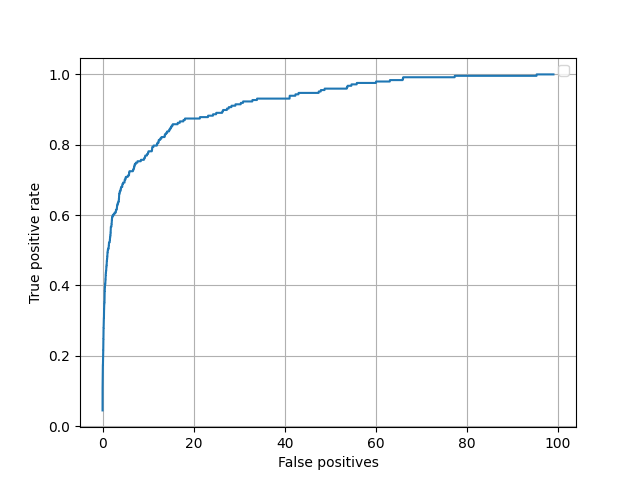
\includegraphics[width=1\columnwidth]{roc.png}
    \caption{ROC curve for the resulting model.}
    \label{fig:roc}
\end{figure}

\section{Conclusion}

While this model seems to perform okay, the decision threshold at \numprint{60}\% true positive rate is already pretty low. This shouldn't be a problem provided that the model scores unknown classes lower than that threshold; however, since the dataset doesn't contain such data, I was unable to evaluate that part.

%\bibliographystyle{IEEEtran}
%\bibliography{bibliography}

\end{document}
